\documentclass[12pt,a4paper]{article}
\usepackage[utf8]{inputenc}
\usepackage{amsmath}
\usepackage{amsfonts}
\usepackage{amssymb}
\usepackage{graphicx}
\usepackage{geometry}
\usepackage{fancyhdr}
\usepackage{xcolor}
\usepackage{tcolorbox}
\usepackage{hyperref}
\usepackage{listings}
\usepackage{tikz}
\usetikzlibrary{shapes,arrows,positioning}

\geometry{margin=1in}
\pagestyle{fancy}
\fancyhf{}
\rhead{BlocTime Protocol}
\lhead{Technical Specification}
\cfoot{\thepage}

\definecolor{primaryblue}{RGB}{0,51,102}
\definecolor{accentgold}{RGB}{218,165,32}
\definecolor{treasurygreen}{RGB}{34,139,34}
\definecolor{codegray}{RGB}{240,240,240}

\lstset{
  backgroundcolor=\color{codegray},
  basicstyle=\ttfamily\small,
  breaklines=true,
  frame=single
}

\title{\Huge\textbf{\textcolor{primaryblue}{BlocTime Protocol}}\\[0.5cm]
\Large\textit{A Unified Staking \& Marketplace Ecosystem}\\[0.3cm]
\large\textcolor{accentgold}{Mathematical Framework \& Implementation}\\[0.2cm]
\normalsize\textit{In the spirit of Einstein's elegant simplicity}}
\author{BlocTime Research Team}
\date{\today}

\begin{document}

\maketitle
\thispagestyle{empty}

\begin{center}
\vspace{2cm}
\textit{"Everything should be made as simple as possible, but not simpler."}\\
--- Albert Einstein
\vspace{1cm}

\textit{"Simplicity is the ultimate sophistication."}\\
--- Leonardo da Vinci
\end{center}

\newpage
\tableofcontents
\newpage

\section{Abstract}

The BlocTime Protocol presents a novel approach to decentralized finance by unifying staking incentives with marketplace revenue sharing. Unlike traditional systems that rely on token inflation or manual treasury management, BlocTime creates a sustainable economic loop where \textbf{all marketplace revenue automatically flows to stakers}, proportional to their commitment.

\subsection{Core Thesis}

We propose that sustainable tokenomics must satisfy three principles:

\begin{enumerate}
    \item \textbf{Revenue Alignment}: Stakers benefit from ecosystem growth
    \item \textbf{Automatic Execution}: No manual intervention required
    \item \textbf{Proportional Fairness}: Rewards scale with commitment
\end{enumerate}

BlocTime achieves all three through elegant smart contract design.

\section{System Architecture}

\subsection{Component Overview}

The protocol consists of four primary smart contracts:

\begin{tcolorbox}[colback=primaryblue!5,colframe=primaryblue,title=Smart Contract Components]
\begin{enumerate}
    \item \textbf{BlocTimeToken}: ERC20 token representing staking commitment
    \item \textbf{BlocTimeStaking}: Core staking logic with multipliers and rewards
    \item \textbf{BlocTimeRegistry}: Module metadata and ownership management
    \item \textbf{BlocTimeMarketplaceV3}: Rental marketplace with fractional listings
\end{enumerate}
\end{tcolorbox}

\subsection{Integration Architecture}

\begin{center}
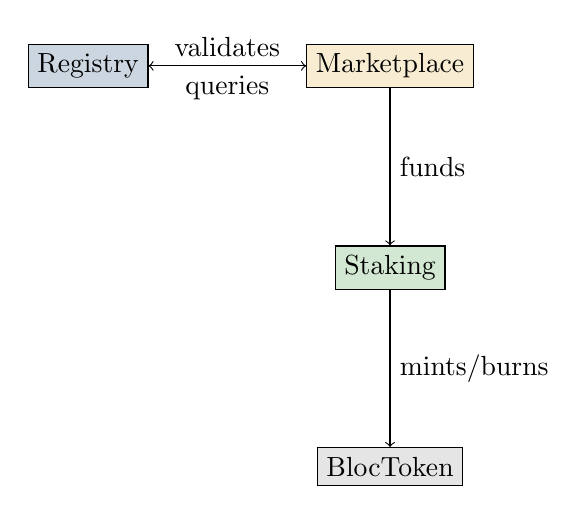
\begin{tikzpicture}[node distance=2cm, auto]
  \node[draw, rectangle, fill=primaryblue!20] (registry) {Registry};
  \node[draw, rectangle, fill=accentgold!20, right=of registry] (marketplace) {Marketplace};
  \node[draw, rectangle, fill=treasurygreen!20, below=of marketplace] (staking) {Staking};
  \node[draw, rectangle, fill=gray!20, below=of staking] (token) {BlocToken};
  
  \draw[->] (marketplace) -- node {queries} (registry);
  \draw[->] (marketplace) -- node {funds} (staking);
  \draw[->] (staking) -- node {mints/burns} (token);
  \draw[->] (registry) -- node {validates} (marketplace);
\end{tikzpicture}
\end{center}

\section{Mathematical Framework}

\subsection{BlocTime Token Minting}

When a user stakes amount $S$ for duration $D$ blocks, they receive BlocTime tokens:

\begin{tcolorbox}[colback=primaryblue!5,colframe=primaryblue,title=Fundamental Minting Equation]
\begin{equation}
\boxed{B_{\text{earned}} = S \cdot M(D)}
\end{equation}

Where:
\begin{itemize}
    \item $B_{\text{earned}}$ = BlocTime tokens minted
    \item $S$ = Stake amount (native tokens)
    \item $M(D)$ = Multiplier function of lock duration $D$
\end{itemize}
\end{tcolorbox}

\subsection{Multiplier Function}

The multiplier function $M(D)$ is defined by a set of monotonic points:

\begin{equation}
P = \{(d_0, m_0), (d_1, m_1), \ldots, (d_n, m_n)\}
\end{equation}

With constraints:
\begin{align}
d_0 < d_1 < \cdots < d_n &\quad \text{(strictly increasing blocks)} \\
m_0 \leq m_1 \leq \cdots \leq m_n &\quad \text{(non-decreasing multipliers)} \\
m_i \geq 10000 &\quad \text{(minimum 1x, in basis points)}
\end{align}

\subsubsection{Linear Interpolation}

For lock duration $D$ where $d_i \leq D \leq d_{i+1}$:

\begin{tcolorbox}[colback=accentgold!5,colframe=accentgold,title=Interpolation Formula]
\begin{equation}
\boxed{M(D) = m_i + \frac{(m_{i+1} - m_i) \cdot (D - d_i)}{d_{i+1} - d_i}}
\end{equation}
\end{tcolorbox}

\textbf{Example Configuration:}

\begin{center}
\begin{tabular}{|c|c|c|}
\hline
\textbf{Blocks} & \textbf{Multiplier (bps)} & \textbf{Multiplier (x)} \\
\hline
0 & 10000 & 1.0x \\
10,000 & 15000 & 1.5x \\
50,000 & 20000 & 2.0x \\
100,000 & 30000 & 3.0x \\
\hline
\end{tabular}
\end{center}

\subsection{Treasury Reward Distribution}

Rewards are distributed proportionally to BlocTime token holdings:

\begin{tcolorbox}[colback=treasurygreen!5,colframe=treasurygreen,title=Reward Distribution Equation]
\begin{equation}
\boxed{R_u = \frac{B_u}{B_{\text{total}}} \cdot T \cdot \frac{\delta}{10000}}
\end{equation}

Where:
\begin{itemize}
    \item $R_u$ = User's claimable rewards
    \item $B_u$ = User's BlocTime token balance
    \item $B_{\text{total}}$ = Total BlocTime tokens in circulation
    \item $T$ = Current treasury balance
    \item $\delta$ = Distribution percentage (basis points)
\end{itemize}
\end{tcolorbox}

\subsection{Marketplace Fee Structure}

\subsubsection{Primary Market (Rentals)}

For a rental of $N$ blocks at price $P$ per block:

\begin{align}
C_{\text{total}} &= N \cdot P \\
F_{\text{treasury}} &= C_{\text{total}} \cdot \frac{\phi}{10000} \\
P_{\text{owner}} &= C_{\text{total}} - F_{\text{treasury}}
\end{align}

Where $\phi$ is the treasury fee in basis points (e.g., 250 = 2.5\%).

\subsubsection{Secondary Market (Resales)}

For a listing sold at price $L$:

\begin{align}
F_{\text{treasury}} &= L \cdot \frac{\phi}{10000} \\
P_{\text{seller}} &= L - F_{\text{treasury}}
\end{align}

\subsection{Fractional Rental Mathematics}

The marketplace supports fractional rental listings defined by block ranges:

\begin{tcolorbox}[colback=primaryblue!5,colframe=primaryblue,title=Fractional Listing]
A rental $R$ with paid blocks $N$ can be listed as:
\begin{equation}
L = (R, b_{\text{from}}, b_{\text{to}}, p)
\end{equation}

Where:
\begin{itemize}
    \item $0 \leq b_{\text{from}} < b_{\text{to}} \leq N$
    \item $p$ = listing price
    \item No overlapping listings allowed
\end{itemize}
\end{tcolorbox}

\textbf{Overlap Detection:}

Two listings $L_1 = (b_1^{\text{from}}, b_1^{\text{to}})$ and $L_2 = (b_2^{\text{from}}, b_2^{\text{to}})$ overlap if:

\begin{equation}
b_1^{\text{from}} < b_2^{\text{to}} \land b_2^{\text{from}} < b_1^{\text{to}}
\end{equation}

\section{Economic Model}

\subsection{Revenue Flow Diagram}

\begin{center}
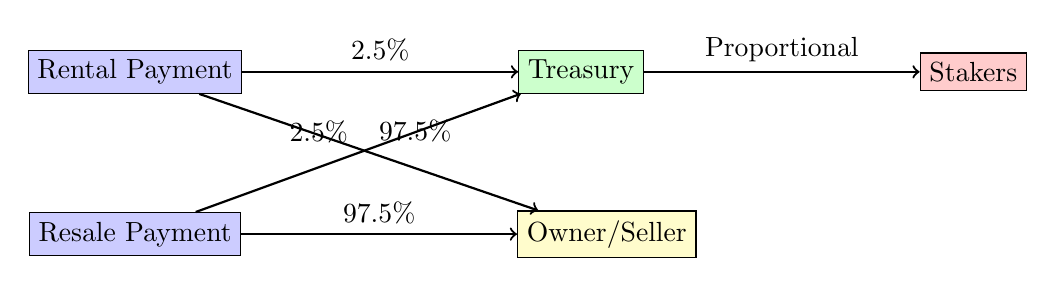
\begin{tikzpicture}[node distance=1.5cm, auto]
  \node[draw, rectangle, fill=blue!20] (rental) {Rental Payment};
  \node[draw, rectangle, fill=blue!20, below=of rental] (resale) {Resale Payment};
  \node[draw, rectangle, fill=green!20, right=of rental, xshift=2cm] (treasury) {Treasury};
  \node[draw, rectangle, fill=yellow!20, right=of resale, xshift=2cm] (owner) {Owner/Seller};
  \node[draw, rectangle, fill=red!20, right=of treasury, xshift=2cm] (stakers) {Stakers};
  
  \draw[->, thick] (rental) -- node {2.5\%} (treasury);
  \draw[->, thick] (rental) -- node {97.5\%} (owner);
  \draw[->, thick] (resale) -- node {2.5\%} (treasury);
  \draw[->, thick] (resale) -- node {97.5\%} (owner);
  \draw[->, thick] (treasury) -- node {Proportional} (stakers);
\end{tikzpicture}
\end{center}

\subsection{Sustainability Analysis}

\textbf{Theorem}: The system is sustainable if marketplace revenue exceeds operational costs.

\textbf{Proof Sketch}:

\begin{enumerate}
    \item Let $R_m$ = total marketplace revenue per period
    \item Let $C_o$ = operational costs per period
    \item Treasury accumulation: $T' = T + \phi \cdot R_m$
    \item Staker rewards: $R_s = T' \cdot \delta / 10000$
    \item If $R_m > C_o$, then $T'$ grows over time
    \item Therefore, $R_s$ grows proportionally
\end{enumerate}

\section{Security Considerations}

\subsection{Smart Contract Security}

\begin{tcolorbox}[colback=red!5,colframe=red,title=Security Measures]
\begin{enumerate}
    \item \textbf{ReentrancyGuard}: All state-changing functions protected
    \item \textbf{SafeERC20}: Safe token transfer operations
    \item \textbf{Access Control}: Owner-only administrative functions
    \item \textbf{Overflow Protection}: Solidity 0.8+ built-in checks
    \item \textbf{Monotonic Enforcement}: Multiplier curve validation
\end{enumerate}
\end{tcolorbox}

\subsection{Economic Attack Vectors}

\subsubsection{Flash Loan Attack}

\textbf{Attack}: Borrow large amount, stake, claim rewards, unstake.

\textbf{Mitigation}: Lock period enforcement prevents immediate unstaking.

\subsubsection{Sybil Attack}

\textbf{Attack}: Create multiple accounts to game rewards.

\textbf{Mitigation}: Rewards proportional to BlocTime, which requires lock commitment.

\subsubsection{Front-running}

\textbf{Attack}: Front-run reward claims to maximize share.

\textbf{Mitigation}: Proportional distribution ensures fairness regardless of claim order.

\section{Implementation Details}

\subsection{Key Functions}

\subsubsection{Staking Contract}

\begin{lstlisting}[language=Solidity]
function stake(uint256 amount, uint256 lockBlocks) external {
    // 1. Transfer tokens from user
    // 2. Calculate multiplier M(lockBlocks)
    // 3. Mint BlocTime = amount * M(lockBlocks)
    // 4. Record stake with start block
}

function unstake() external {
    // 1. Verify lock period elapsed
    // 2. Burn user's BlocTime tokens
    // 3. Return staked tokens
}

function claimRewards() external {
    // 1. Calculate pending rewards
    // 2. Transfer from treasury
    // 3. Update claimed amount
}
\end{lstlisting}

\subsubsection{Marketplace Contract}

\begin{lstlisting}[language=Solidity]
function rent(uint256 moduleId, uint256 blocks) external {
    // 1. Validate module availability
    // 2. Calculate cost and fee
    // 3. Transfer payment from renter
    // 4. Send fee to treasury
    // 5. Send remainder to owner
    // 6. Create rental record
}

function listFractionalForSale(
    uint256 rentalId,
    uint256 fromBlock,
    uint256 toBlock,
    uint256 price
) external {
    // 1. Validate ownership
    // 2. Check no overlapping listings
    // 3. Create listing record
}
\end{lstlisting}

\subsection{Gas Optimization}

\begin{itemize}
    \item \textbf{Packed Storage}: Struct fields optimized for storage slots
    \item \textbf{Batch Operations}: Support for multiple claims/stakes
    \item \textbf{View Functions}: Off-chain calculations where possible
    \item \textbf{Event Indexing}: Efficient event filtering
\end{itemize}

\section{Testing Strategy}

\subsection{Unit Tests}

\begin{enumerate}
    \item \textbf{Staking}: Lock/unlock, multiplier calculation, reward distribution
    \item \textbf{Marketplace}: Rentals, listings, fee collection
    \item \textbf{Registry}: Module registration, updates, deactivation
    \item \textbf{Integration}: Cross-contract interactions
\end{enumerate}

\subsection{Integration Tests}

\begin{enumerate}
    \item \textbf{End-to-End Flows}: Complete user journeys
    \item \textbf{Edge Cases}: Boundary conditions, overflow scenarios
    \item \textbf{Attack Simulations}: Security vector testing
    \item \textbf{Gas Profiling}: Optimization validation
\end{enumerate}

\section{Deployment Guide}

\subsection{Network Configuration}

\begin{center}
\begin{tabular}{|l|l|l|}
\hline
\textbf{Network} & \textbf{Chain ID} & \textbf{RPC URL} \\
\hline
Ganache (Local) & 1337 & http://localhost:8545 \\
Base Mainnet & 8453 & https://mainnet.base.org \\
\hline
\end{tabular}
\end{center}

\subsection{Deployment Sequence}

\begin{enumerate}
    \item Deploy payment token (or use existing)
    \item Deploy BlocTimeStaking with parameters
    \item Deploy BlocTimeRegistry
    \item Deploy BlocTimeMarketplaceV3 with references
    \item Configure multiplier points
    \item Set distribution percentage
    \item Verify all integrations
\end{enumerate}

\section{Future Enhancements}

\subsection{Planned Features}

\begin{enumerate}
    \item \textbf{Governance}: Community voting on parameters
    \item \textbf{Multi-token Support}: Accept various payment tokens
    \item \textbf{Cross-chain Bridges}: Expand to multiple networks
    \item \textbf{NFT Integration}: Represent stakes/rentals as NFTs
    \item \textbf{Advanced Analytics}: On-chain metrics dashboard
    \item \textbf{Automated Market Making}: Dynamic pricing algorithms
\end{enumerate}

\subsection{Research Directions}

\begin{enumerate}
    \item \textbf{Optimal Multiplier Curves}: Game-theoretic analysis
    \item \textbf{Dynamic Fee Adjustment}: Market-responsive fees
    \item \textbf{Liquidity Incentives}: Bootstrap marketplace growth
    \item \textbf{Risk Models}: Quantify economic attack vectors
\end{enumerate}

\section{Conclusion}

The BlocTime Protocol demonstrates that elegant mathematics and robust engineering can create sustainable tokenomics. By automatically directing marketplace revenue to stakers, the system aligns incentives across all participants:

\begin{itemize}
    \item \textbf{Stakers} earn from ecosystem growth
    \item \textbf{Module owners} access liquidity and users
    \item \textbf{Renters} access valuable resources
    \item \textbf{The ecosystem} grows through positive feedback loops
\end{itemize}

\vspace{1cm}

\begin{center}
\textcolor{primaryblue}{\textbf{\Large BlocTime Protocol}}\\
\vspace{0.3cm}
\textcolor{accentgold}{\textit{Where Mathematics Meets Economics}}\\
\vspace{0.3cm}
\textcolor{treasurygreen}{\textit{Powered by Elegant Simplicity}}
\end{center}

\appendix

\section{Appendix A: Contract Addresses}

\subsection{Ganache (Local)}

\begin{lstlisting}
PaymentToken: 0x...
BlocTimeStaking: 0x...
BlocTimeToken: 0x...
BlocTimeRegistry: 0x...
BlocTimeMarketplace: 0x...
\end{lstlisting}

\subsection{Base Mainnet}

\begin{lstlisting}
PaymentToken: 0x...
BlocTimeStaking: 0x...
BlocTimeToken: 0x...
BlocTimeRegistry: 0x...
BlocTimeMarketplace: 0x...
\end{lstlisting}

\section{Appendix B: Gas Costs}

\begin{center}
\begin{tabular}{|l|r|}
\hline
\textbf{Operation} & \textbf{Gas Cost} \\
\hline
Stake & ~150,000 \\
Unstake & ~100,000 \\
Claim Rewards & ~80,000 \\
Rent Module & ~200,000 \\
List Fractional & ~120,000 \\
Buy Listing & ~180,000 \\
\hline
\end{tabular}
\end{center}

\section{Appendix C: References}

\begin{enumerate}
    \item OpenZeppelin Contracts: https://docs.openzeppelin.com/contracts/
    \item Hardhat Documentation: https://hardhat.org/docs
    \item Base Network: https://base.org
    \item EIP-20 (ERC20): https://eips.ethereum.org/EIPS/eip-20
\end{enumerate}

\end{document}
